\chapter{Localização de Placas Veiculares usando Redes Neurais Convolucionais}
	\label{ses:metodo}

O método proposto para a localização de placas envolve uma série de etapas,
conforme ilustrado na figura \ref{fig:etapas_metodo_proposto}.

\begin{figure}[!htb]
	\centering
	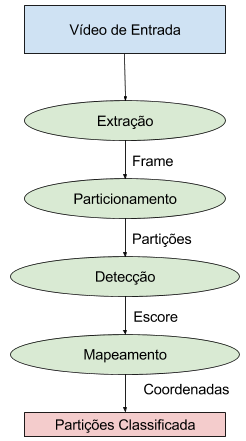
\includegraphics[scale=0.75]{etapas_metodo_proposto.png}
	\caption{Etapas do método proposto para localização de placas veiculares}
	\label{fig:etapas_metodo_proposto}
	(próprio autor).
\end{figure}

O processo ``extração'' é responsável por obter as \emph{frames} do vídeo.
Uma \emph{frame} é equivalente a uma imagem 2D, e pode ser representada por
tensores de dimensões \sigla{HWC}{\emph{Height X Width X Channel}, altura X
largura X
canal} (altura, largura e canais de cor). Todos os \emph{frames} de um mesmo
vídeo geram tensores do mesmo tamanho.

O processo ``particionamento'' toma como entrada uma \emph{frame} do
vídeo e gera
múltiplas sub imagens aqui denominadas ``partições'', geradas através de um
recorte retangular de \emph{pixels} contíguos. As partições têm dimensões
compatíveis com a rede neural que será usada no passo seguinte.

A etapa denominada ``detecção'' é, mais especificamente, uma rede neural
artificial convolucional profunda treinada para modelar uma função escalar cujo
valor, denominado ``escore'', é determinado pela presença e posição, ou não
presença, de uma placa veicular.

A etapa ``mapeamento'' recebe todos os escores calculados para todas as
partições da imagem e calcula a partir delas as coordenadas dos centros das
placas. Quando uma placa está perfeitamente centrada em uma partição esta terá
valor 1, enquanto todas as vizinhas terão o valor 0. Quando o centro da placa
está entre duas partições então ambas terão valor superior a zero. A
implementação usada aqui considera apenas o maior valor. A posição do centro da
placa é estimado como sendo a posição do centro da partição onde ela foi
detectada. Portanto a resolução deste módulo é igual metade da largura da
partição em $X$ e metade da altura em $Y$.

O método aqui proposto inclui algumas opções na implementação do processo
supradescrito. Elas dizem respeito:

\begin{itemize}
\item ao tamanho das partições de imagem a serem recortadas e, por
	consequência, ao tamanho da entrada da rede neural;
\item à escolha do \emph{stride} das partições da rede neural;
\item à escolha da função que a rede neural está modelando;
\item à escolha da arquitetura e dos hiperparâmetros da rede neural.
\end{itemize}

\section{Tamanho das Partições}
O tamanho das partições define as dimensões do tensor da rede neural, portanto
o tamanho do seu ``campo visual''.


\begin{figure}[!htb]
	\centering
	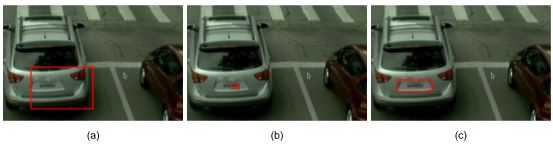
\includegraphics{ex_tres_segmentos.png}
	\caption{Exemplo de três tamanhos de partições}
	\label{fig:ex_tres_segmentos}
	Em (a) a partição possui um grande campo visual, porém tem baixa precisão.
	Em (b) há um campo visual muito pequeno para permitir que a rede neural
	opere corretamente. A terceira é apropriada, pois é relativamente pequena e
	inclui a placa inteira e vários \emph{pixels} adicionais, permitindo que a
	rede neural aprenda o contraste entre placa e o fundo (próprio autor).
\end{figure}

Quanto maior o campo visual da rede neural, mais dados ela vai ter para
processar, porém menor será a precisão. Se o campo visual for muito pequeno,
como na figura \ref{fig:ex_tres_segmentos}b a precisão seria maximizada,
mas a área não é suficiente para a rede neural operar corretamente. Se
o campo visual for muito grande, como na figura \ref{fig:ex_tres_segmentos}a,
a rede neural terá mais características para usar, mas a precisão da
localização será muito prejudicada.

De forma geral, as dimensões das partições devem ser minimizadas, mas deve-se
garantir que a placa caiba no seu interior, com um pouco de
sobra. As figuras \ref{fig:ex_tres_segmentos}c e \ref{fig:ex_placa} mostram
um bom tamanho. A região adicional fora da placa vai servir para a rede
neural aprender que existe um contraste de \emph{features} entre o
interior e o exterior da placa. Este contraste vai ser usado não só para
identificar quando existe uma placa, mas também para excluir muitos casos de
falsos positivos, como \emph{banners} e outros textos que podem ser
encontrados em veículos.

\begin{figure}[!htb]
	\centering
	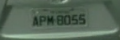
\includegraphics{ex_placa.png}
	\caption{Exemplo de partição com bom tamanho}
	\label{fig:ex_placa}
	(próprio autor).
\end{figure}

\section{\emph{Strides} das Partições}
A abordagem que está sendo proposta envolve usar um detector para construir um
localizador. Uma implementação ingênua desta abordagem seria treinar o detector
para detectar placas de trânsito que estejam centradas na sua entrada e aplicar
este detector como descrito na sessão \ref{sec:localiz_objetos}, usando
\emph{stride} $1 \times 1$.  Isso iria requerer aplicar a rede neural centrada
em cada \emph{pixel} da imagem. Se for feita a aplicação de um detector com
campo visual $D_1 \times D_2$ em uma \emph{frame} com dimensões $F_1 \times
F_2$ com \emph{stride} $1 \times 1$ sem estender as bordas pode-se demonstrar
que o detector terá que ser aplicado $N$ vezes, onde:

\begin{equation}
	N = (F_1 - D_1 + 1) \cdot (F_2 - D_2 + 1)
\end{equation}

Para um detector com dimensões \sigla{HW}{\emph{Height X width}, altura X
largura} de $40 \times 120$ em uma imagem
$480 \times 768$ seriam geradas 286.209 partições, e cada uma delas precisaria
ser aplicada ao detector, o que é proibitivo.

Para resolver este problema propõe-se o uso de um \emph{stride} de
$50\% \times 50\%$ do tamanho da partição. Isso significa que duas amostras
consecutivas (lado-a-lado) tem os seus centros a uma distância igual a sua
largura sobre dois, gerando partições como as ilustradas na figura
\ref{fig:ex_3_segmentos}.

\begin{figure}[!htb]
	\centering
	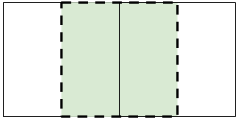
\includegraphics[scale=0.8]{ex_3_segmentos.png}
	\caption{Ilustração de 3 partições sucessivas}
	\label{fig:ex_3_segmentos}
	Observar que o centro de uma partição está contido no perímetro das
	partições vizinhas (próprio autor).
\end{figure}

Uma propriedade dessa escolha é que o centro de uma partição de imagem está
contido no perímetro de todas as partições vizinhas. Esta propriedade é
justamente o objetivo do \emph{stride} de 50\%, conforme será descrito na
sessão \ref{ses:funcao_a_modelar}.

O número de partições na direção da altura será $T_H$, e na largura será
$T_W$, sendo:

\begin{equation}
	T_H=\left\lfloor \frac{2F_1}{D_1}-1 \right\rfloor \\
\end{equation}

\begin{equation}
	T_W=\left\lfloor \frac{2F_2}{D_2}-1 \right\rfloor \\
\end{equation}

E o número de partições a serem classificadas será:

\begin{equation}
	N=\left\lfloor \frac{2F_1}{D_1}-1 \right\rfloor \cdot
		\left\lfloor \frac{2F_2}{D_2}-1 \right\rfloor
\end{equation}

Tomando o mesmo caso calculado anteriormente (detector $40 \times 120$ em
\emph{frames} $480 \times 768$ sem extensão de borda) com a estratégia proposta
de particionamento o número de partições a serem classificadas cai de 286.209
para $23 \cdot 11=253$.

\section{Função a ser Modelada} \label{ses:funcao_a_modelar}

A rede neural vai ser treinada para modelar o valor de uma função $P$ que
leva um tensor que representa uma partição da \emph{frame} a um real no
intervalo $[0;1]$:

\begin{equation}
	P:S \to [0;1] \in \mathbb{R} 
\end{equation}

O valor dessa função é resultante da presença de uma placa veicular. Devido ao
fato de que o particionamento será feito com \emph{stride} maior que 1 não há
garantia de que a placa estará centralizada, e ainda assim a função precisa
identificar que ela está presente.

A função proposta foi construída baseada na forma com que a placa veicular
passa de uma partição para a partição vizinha. A função deve possuir as
seguintes características:

\begin{itemize}
\item a função é contínua quando uma placa é deslocada de forma contínua na
	entrada por qualquer caminho;
\item quando a placa veicular está no centro de uma partição a função de
	saída deve ser 1, e quando está no centro da partição vizinha deve ser 0;
\item uma, e apenas uma partição deve possuir valor 1 como consequência da
	presença da placa, exceto nos pontos críticos, na vizinhança dos quais a
	função é menor que 1.
\end{itemize}

A figura \ref{fig:placa_movida_entre_segmentos} ilustra os pontos principais
quando uma placa é movida horizontalmente entre duas partições.

\begin{figure}[!htb]
	\centering
	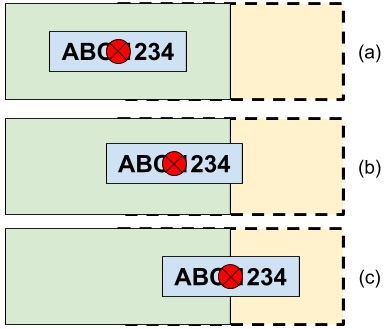
\includegraphics[scale=0.6]{placa_movida_entre_segmentos.png}
	\caption{Placa veicular sendo movida entre duas partições}
	\label{fig:placa_movida_entre_segmentos}
	Ilustração dos pontos críticos para a definição da função a ser modelada
	pela rede neural, mostrando duas partições vizinhas, uma pintada de verde e
	o outro amarelo com borda pontilhada. Em (a) a placa está centrada na
	partição da esquerda e no perímetro da partição da direita.
	Em (b) o centro da placa está no meio caminho entre os centros dos duas
	partições. Em (c) o centro da placa está no centro da partição da direita e
	perímetro da partição da esquerda (próprio autor).
\end{figure}

A figura \ref{fig:func_a_modelar_2_seg} mostra o valor da função para
duas partições vizinhas à medida que a placa é movida. Pode-se observar que
apenas um das partições possui valor 1 por vez, exceto no ponto cuja vizinhança
é menor que 1. Também observa-se
que quando a placa está centrada em uma partição, a função possui valor zero
na outra partição.

\begin{figure}[!htb]
	\centering
	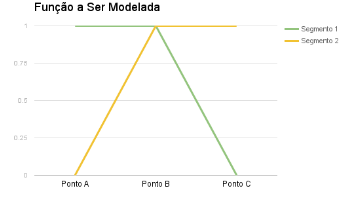
\includegraphics[scale=0.75]{func_a_modelar_2_seg.png}
	\caption{Valor da função em duas partições a medida que a placa se move
	entre elas}
	\label{fig:func_a_modelar_2_seg}
	Observa-se que valor da saída da função para duas partições a medida que a
	placa é movida do centro da partição 1 (o da esquerda) para a partição 2 (a
	da direita) (próprio autor).
\end{figure}

\begin{figure}[!htb]
	\centering
	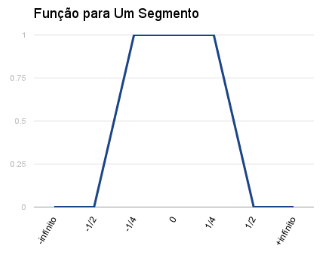
\includegraphics[scale=0.75]{func_a_modelar_1_seg.png}
	\caption{Valor da função a modelar, de $\infty$ a $+\infty$}
	\label{fig:func_a_modelar_1_seg}
	Observa-se que o valor da variável dependente a em medida que a placa
	é deslocada desde $-\infty$ até $+\infty$ da esquerda para a direita,
	enquanto a mesma está centrada na altura. A abscissa é a distância
	normalizada entre os centros da partição e da placa (próprio autor).
\end{figure}

Na figura \ref{fig:func_a_modelar_1_seg} observa-se o valor de uma função
quando a placa está alinhada na altura e é deslocada horizontalmente. Como
a abscissa é a distância normalizada entre os centros obtém-se o valor 0,5
quando o centro da placa está a uma distância igual a metade do tamanho da
partição para a direita, como ilustrado na figura
\ref{fig:placa_movida_entre_segmentos}c.

No caso de uma placa alinhada na direção $y$ (distância em $y$ é 0), e sendo
deslocada apenas em $x$, variando a distância normalizada $\Delta x$, a função
proposta é:

\begin{equation}
	f_x(\Delta x) = \begin{cases}
		1 \text{, se } |\Delta x| \leq 1/4
		\\
		\frac{1/2-|\Delta x|}{1/2-1/4} \text{, se } 1/4<|\Delta x|<1/2
		\\
		0 \text{, se } |\Delta x| \geq 1/2
	\end{cases}
\end{equation}

Da maneira semelhante, quando a distância em x é zero e a distância 
normalizada $\Delta y$ é livre:

\begin{equation}
	f_y(\Delta x) = \begin{cases}
		1 \text{, se } |\Delta y| \leq 1/4
		\\
		\frac{1/2-|\Delta y|}{1/2-1/4} \text{, se } 1/4<|\Delta y|<1/2
		\\
		0 \text{, se } |\Delta y| \geq 1/2
	\end{cases}
\end{equation}

Quando usado com as direções x e y livres a função a ser estimada pela rede
neural é:

\begin{equation} \label{eq:funcao_a_modelar}
	f=f_x \cdot f_y
\end{equation}

O gráfico \emph{3D} desta função está representado na figura
\ref{fig:func_a_modelar_3d}, mostrando o
efeito simultâneo dos eixos $x$ e $y$.  Observa-se que quando a placa
está com o seu centro a uma distância normalizada inferior 1/4 em $x$ e em $y$
simultaneamente, a função vai produzir o valor 1. O gráfico não possui
descontinuidades. Quando a distância normalizada supera 1/2 em qualquer
direção o valor da função é 0.

\begin{figure}[!htb]
	\centering
	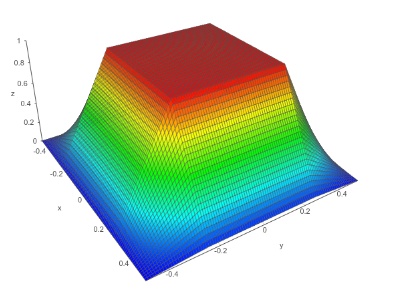
\includegraphics[scale=0.75]{func_a_modelar_3d.png}
	\caption{Gráfico 3D da função à modelar}
	\label{fig:func_a_modelar_3d}
	Gráfico da função que a rede neural deve modelar. As abscissas representam
	a distância normalizada entre o centro da partição e da placa em cada
	direção (próprio autor).
\end{figure}


\section{Arquitetura da Rede Neural}

A arquitetura da rede neural, incluindo seus hiperparâmetros, deve ser
escolhida de forma a balancear desempenho de classificação com tempo de
propagação. Se a rede neural requerer muitas operações, pode aumentar o
desempenho de classificação, mas o tempo de processamento vai aumentar.
Idealmente a rede neural deve ser restrita a um tamanho que permita que todos
as partições da imagem sejam classificadas de forma que o sistema como um todo
entregue a taxa de \emph{frames} desejada para a resolução do vídeo necessária
e hardware disponíveis onde a solução vai ser implantada.

Na implementação da rede neural convolucional existem otimizações que podem ser
feitas para reduzir o número de operações enquanto mantendo ou reduzindo pouco
a capacidade da rede neural de executar a operação para a qual vai ser
treinada. Estas otimizações são um campo ativo de pesquisa, sendo relevantes os
\emph{papers} produzidos como resultado da competição \emph{ImageNet Large
Scale Visual Recognition Competition (ILSVRC)}. Os \emph{papers}
\cite{szegedy2015going} e \cite{szegedy2015rethinking},
por exemplo, detalham várias substituições que podem ser feitas para este fim.


